\documentclass[11pt,a4paper]{article}
\usepackage[margin=2.25cm,headheight=22pt]{geometry}
\usepackage[T1]{fontenc}\usepackage[utf8]{inputenc}\usepackage[spanish]{babel}
\usepackage{lmodern,microtype,graphicx,xcolor,fancyhdr,titlesec,tabularx,booktabs,hyperref,xurl}
\definecolor{azul}{HTML}{18324B}\definecolor{turquesa}{HTML}{087E83}\definecolor{gris}{HTML}{52616B}
\pagestyle{fancy}\fancyhf{}\fancyhead[L]{\small Unidad 6 | Ejercicio 1}\fancyhead[R]{\small Juan Skobalski}\fancyfoot[C]{\thepage}
\titleformat{\section}{\Large\bfseries\color{azul}}{}{0pt}{}\titleformat{\subsection}{\large\bfseries\color{turquesa}}{}{0pt}{}
\setlength{\parindent}{0pt}\setlength{\parskip}{8pt}\renewcommand{\arraystretch}{1.5}
\hypersetup{pdftitle={Guía de Autoprotección Digital},pdfauthor={Juan Skobalski},colorlinks=true,urlcolor=turquesa}
\begin{document}
\thispagestyle{empty}\vspace*{1cm}
{\large\color{turquesa}C O D E R H O U S E}\par\rule{\textwidth}{0.5pt}\vspace{2cm}
{\Large\color{gris}CIBERSEGURIDAD}\par
{\Huge\bfseries\color{azul}Guía de\\Autoprotección Digital}\par
\vspace{0.7cm}{\LARGE\color{turquesa}Navegación privada, extensiones y VPN}\par
\vspace{1cm}Unidad 6 | Ejercicio 1
\vfill
\begin{tabularx}{\textwidth}{lX}
\textbf{Estudiante} & Juan Skobalski\\
\textbf{Curso} & Ciberseguridad\\
\textbf{Navegador} & Zen, basado en Firefox\\
\textbf{Extensión} & Privacy Badger (EFF)\\
\textbf{Fecha} & 11 de noviembre de 2026
\end{tabularx}
\vspace{1cm}\par Privacidad local, protección del tráfico y límites de cada herramienta.
\clearpage
\section{Introducción y alcance}
El ejercicio combina navegación privada en Zen, Privacy Badger y una prueba con VPN. Su objetivo es distinguir la privacidad local de la protección de la conexión y aplicar estos conceptos a una operación bancaria desde Wi-Fi público.

La captura acredita el modo privado y la extensión activa. La revisión del historial y la realización de la prueba con VPN fueron confirmadas por el estudiante. No se aportaron IP, proveedor, servidor ni capturas de esa comparación; no se atribuyen valores o ubicaciones específicos.
\section{Cuadro comparativo}
\small
\begin{tabularx}{\textwidth}{p{2.4cm}XX}
\toprule\textbf{Aspecto} & \textbf{Modo privado} & \textbf{VPN}\\\midrule
Historial local & No incorpora las visitas privadas al historial habitual. & No impide que el navegador guarde el historial.\\
Dirección IP & No cambia la IP pública por activar este modo. & El sitio normalmente observa la IP de salida del servidor para el tráfico del túnel.\\
Cifrado de datos & No agrega un túnel. HTTPS funciona también fuera del modo privado. & Cifra entre el equipo y el servidor VPN; HTTPS sigue protegiendo la comunicación con el sitio.\\
Cookies & Descarta las cookies de la sesión privada al finalizarla. & No elimina cookies ni sesiones del navegador.\\
Observación de red & No oculta por sí mismo los metadatos al ISP o a la red local. & Reduce su visibilidad del tráfico dentro del túnel; aún observan conexión VPN, tiempos y volumen.\\
Identificación & Iniciar sesión permite al servicio reconocer al usuario. & La cuenta identifica al usuario aunque cambie su IP.\\\bottomrule
\end{tabularx}\normalsize
\subsection{Límites}
El modo privado no elimina descargas ni garantiza ausencia de rastros en todo el sistema. Una VPN depende del enrutamiento, posibles fugas y confianza en su proveedor. Las cuentas y la huella del navegador pueden permitir correlación. Privacy Badger reduce determinadas formas de seguimiento; no sustituye una VPN ni cifra todo el tráfico.
\clearpage
\section{Práctica y evidencia visual}
Se utilizó Zen, basado en Firefox. Privacy Badger aparece fijado en la barra y funcionando en una ventana privada. La imagen muestra Google Maps como página de prueba.
\begin{center}
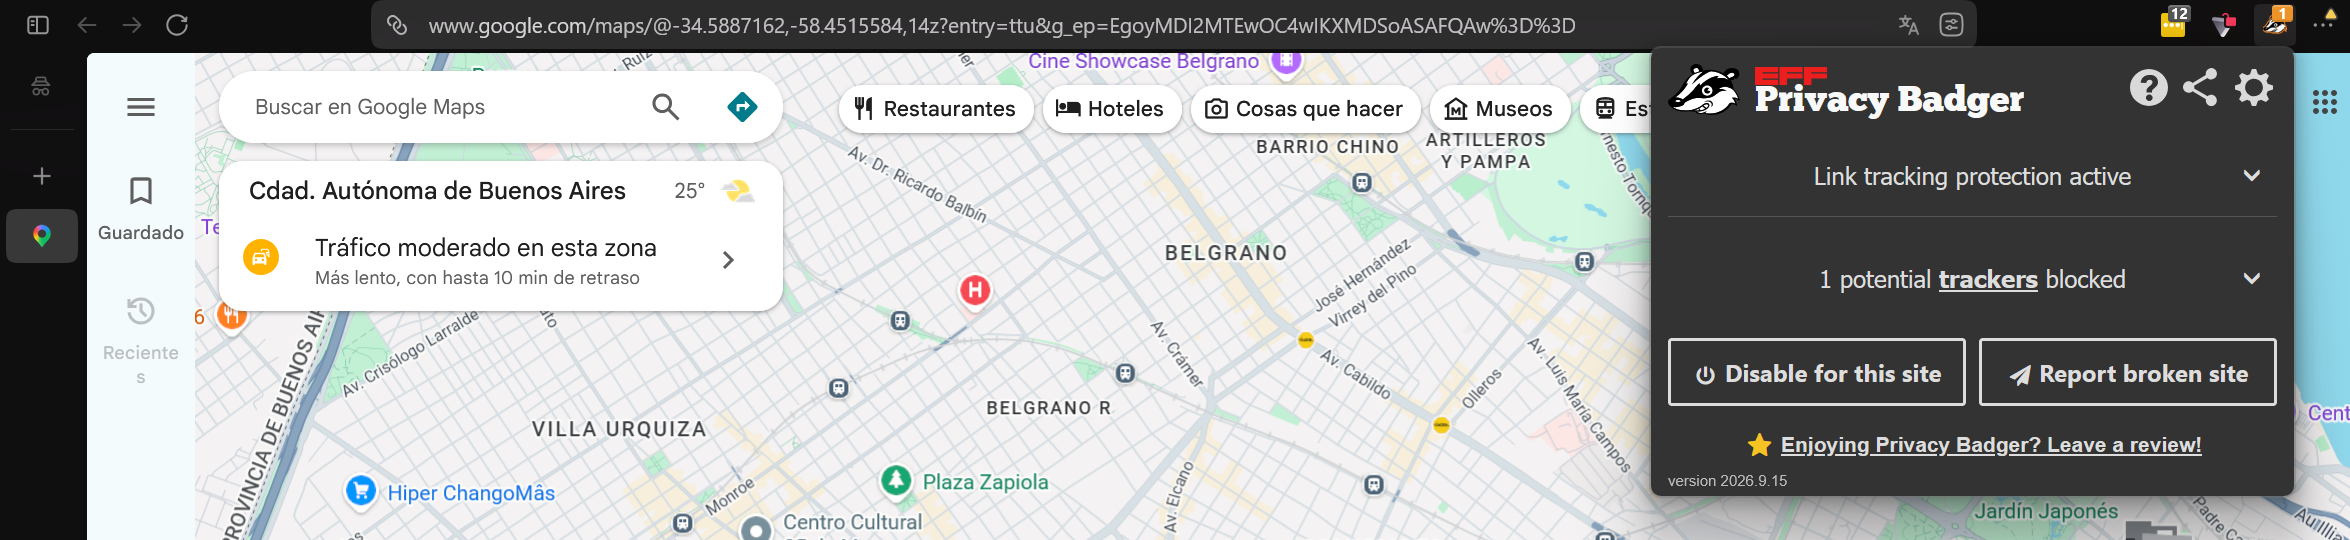
\includegraphics[width=\textwidth]{capturas/01_privado_extension.png}
\par\small\color{gris}Figura 1. Ventana privada de Zen y panel de Privacy Badger activo.
\end{center}
\subsection{Lectura de la evidencia}
El indicador de navegación privada está en el lateral izquierdo. El icono de Privacy Badger se encuentra en la barra superior. Su panel informa protección de enlaces activa y un posible rastreador bloqueado. El botón para desactivar la extensión en el sitio es coherente con su estado activo. La versión visible es 2026.9.15.

La captura no acredita una conexión VPN ni ausencia completa de rastreo. Las coordenadas visibles corresponden a la vista del mapa y no prueban la ubicación física del estudiante.
\subsection{Configuración reproducible}
En \texttt{about:addons} se permite que Privacy Badger funcione en ventanas privadas. Desde el menú de extensiones se utiliza \textit{Pin to Toolbar}. Se abre una ventana privada con Ctrl + Shift + P, se visita el sitio y se consulta el panel.
\subsection{Resultados registrados}
\begin{tabularx}{\textwidth}{p{4cm}X}
\toprule\textbf{Prueba} & \textbf{Resultado y soporte}\\\midrule
Modo privado y extensión & Visibles en la figura 1.\\
Historial tras cerrar & El estudiante confirmó que la visita privada no se agregó al historial. Resultado declarado, sin captura adicional.\\
Prueba con VPN & El estudiante confirmó haberla realizado. No se documentaron las IP de origen y salida ni una ubicación concreta.\\\bottomrule
\end{tabularx}
\clearpage
\section{Análisis de caso}
\subsection{¿Es seguro entrar a mi banco en un Starbucks solo usando modo incógnito?}
El modo incógnito por sí solo no permite considerar segura la operación: limita el almacenamiento local, pero no verifica la legitimidad de la red ni añade cifrado. Una red pública puede ser suplantada o permitir observación del tráfico y sus metadatos.

El riesgo de \textit{sniffing} depende del protocolo. HTTP transmite información sin cifrar a nivel de aplicación. HTTPS correctamente validado protege el contenido y las credenciales frente a la escucha pasiva. Compartir el Wi-Fi no basta para leer una contraseña enviada mediante HTTPS. El ISP puede observar metadatos y, según los mecanismos utilizados, inferir destinos; eso no significa que vea el contenido completo de cada página cifrada.

Persisten riesgos como phishing, certificados inválidos ignorados y equipos comprometidos. Una VPN confiable añade protección en el tramo de la red pública, pero no convierte un sitio falso en legítimo ni reemplaza HTTPS.
\subsection{Conducta propuesta}
Para una operación sensible utilizaría la aplicación o dirección oficial del banco, mantendría el sistema actualizado, usaría MFA y preferiría una conexión propia si estuviera disponible. Si utilizara VPN, comprobaría que estuviera conectada y que el tráfico relevante pasara por ella. No ignoraría advertencias de certificados para completar la operación.
\section{Conclusión}
El modo privado limita el registro local de la sesión, Privacy Badger reduce el seguimiento y la VPN protege el tráfico enrutado hasta su servidor. Son controles complementarios con límites distintos. Las cuentas personales y las decisiones del usuario siguen influyendo en su identificación y seguridad.
\subsection{Referencias}
\small
\begin{itemize}
\item Zen: \url{https://docs.zen-browser.app/user-manual/extensions}
\item Mozilla: \url{https://support.mozilla.org/en-US/kb/private-browsing-use-firefox-without-history}
\item EFF: \url{https://privacybadger.org/}
\end{itemize}
\end{document}
